\documentclass[12pt,a4paper]{article}
\usepackage{CJKutf8}
\usepackage{setspace}
\onehalfspacing
\usepackage{graphicx, subfig} % Required for inserting images
\usepackage{sectsty} % for section name format in center
\usepackage[table,xcdraw]{xcolor}%表格
\usepackage{float}
\usepackage{hyperref}

\textwidth      = 137.0mm
\textheight     = 224.0mm
\topmargin      =  -3.0mm
\headheight     =   0.0mm
\headsep        =  10.0mm
\footskip       =   8.0mm
\oddsidemargin  =  10.6mm
\evensidemargin =  10.6mm
\hoffset = -0.2cm

\begin{document}
\begin{CJK*}{UTF8}{bsmi} % 定義中文環境
\sectionfont{\centering}
\begin{center}
    \textbf{\fontsize{24}{32}\selectfont 中原大學}\\
    \textbf{\fontsize{24}{32}\selectfont OOOO學系}\\
    \textbf{\fontsize{24}{32}\selectfont O士OOOO}\\
    \textbf{} \\
    \textbf{} \\
    \textbf{} \\ 
    \textbf{} \\
    \textbf{\fontsize{18}{21.6}\selectfont 中文論文範本}\\
    \textbf{\fontsize{18}{21.6}\selectfont This is a thesis template.}\\
    \textbf{} \\
    \textbf{} \\
\end{center}
\begin{center}
    \textbf{} \\
    \textbf{} \\
    \textbf{} \\
    \textbf{} \\
    \textbf{} \\
    \textbf{} \\
    \textbf{} \\
    \textbf{\fontsize{24}{32}\selectfont 指導教授:OOO} \\
    \textbf{\fontsize{24}{32}\selectfont 研究生:OOO} \\
\end{center}
\vfill
\begin{center}
    \textbf{\fontsize{24}{21.6}\selectfont 中華民國113年O月}
\end{center}
\thispagestyle{empty}
\clearpage

\pagenumbering{Roman} %以下頁碼使用大寫羅馬數字
\input{abstract_Chinese.tex}

\section*{Abstract}
\addcontentsline{toc}{section}{Abstract}
In 1953, a group of Christian educators and local gentries got together to establish an agricultural and engineering college in Taiwan to train science and engineering talent in the Christian spirit. After several name changes and long preparations, the Chung Yuan Christian College of Science and Engineering (CYCC) was established in October 1955 upon approval by the Ministry of Education. With "education through honest, diligent pursuit and practical experience" as the school`s motto, the College was composed of four departments, namely, the departments of physics, chemistry, chemical engineering, and civil engineering. Upgraded to the status of a full university, CYCC was renamed Chung Yuan Christian University (CYCU) on Aug. 1, 1980. 
\par
After five decades, CYCU has developed with support from all members of the Board of Trustees, as well as immense contributions from past presidents and administrators, Kuo Ke-tee, Hsieh Ming-shan, Han Wei, Yuan Ta-nien, Yin Shiu-hau, Chang Kwang-cheng , Hsiung Shen-kan, and Cheng Wan-lee who represents stages in CYCU creation, foundation, growth, steadfastness, and expansion. The University enrolls students in seven-granting school and colleges, such as the College of Science, Engineering, Business, Design, Electrical Engineering and Computer Science, Humanities and Education, and the School of Law. The university offers 38 graduate programs and 13 Ph.D. programs in 29 departments. There are more than 120,000 alumni and most of them devote their best to the progress of society. 
\par
\clearpage

\addcontentsline{toc}{section}{謝辭}
\begin{center}
    \textbf{\fontsize{18}{21.6}\selectfont 謝辭} \\
\end{center}
中原大學之建校，本基督愛世之忱，\\
以信、以望、以愛，致力於中國之高等教育，\\
旨在追求真知力行，以傳啟文化、服務人類。
\clearpage

\addcontentsline{toc}{section}{目錄}
\renewcommand{\contentsname}{目錄} %將latex自帶的"Contents"名稱改為 "目錄"
\tableofcontents
\clearpage

\renewcommand{\listfigurename}{圖目錄}
\listoffigures
\addcontentsline{toc}{section}{圖目錄}
\clearpage

\renewcommand{\listtablename}{表目錄}
\addcontentsline{toc}{section}{表目錄}
\listoftables
\clearpage

\pagenumbering{arabic} %以下頁碼使用阿拉伯/印度數字

\section*{第一章\ 論文格式與目錄設定}
\addcontentsline{toc}{section}{第一章\ 論文格式與目錄設定}

\subsection*{1.1\ 標號}
\addcontentsline{toc}{subsection}{1.1\ 標號}
插入圖片之後，在要加上編號的地方，點選「參考資料」/「標號」/「插入標號」。第一次新增標號時，要點選「新增標籤」，輸入「圖」或「表」，之後只要在標籤裡選擇「圖」或「表」即可，如果有設定好大綱編號，可以在編號方式中將「包含章節編號」打勾，在這個範本第幾章是使用標題1，所以章節起始樣式選標題1，按確定，插入標號後，按一下tab (不要使用空白，以免影響到圖目錄的對齊)，接著在後面打上想要的說明即可。
\textbf{}\\
\begin{figure}[h]
    \centering
    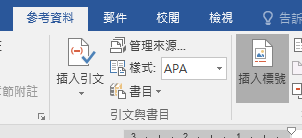
\includegraphics[width=.8\textwidth]{figure1.png} %圖片文件的路徑
    \addcontentsline{lof}{figure}{Figure1.1\ 插入標號的路徑} 
    \caption*{Figure1.1\ 插入標號的路徑}
    \label{img} 
\end{figure}
\begin{figure}[h]
    \centering %置中
    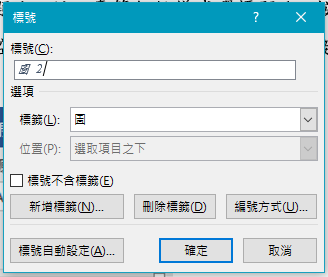
\includegraphics[width=.8\textwidth]{figure2.png}
    \addcontentsline{lof}{figure}{Figure1.2\ 標號設定} 
    \caption*{Figure1.2\ 標號設定} 
    \end{figure}
\clearpage

\subsection*{1.2\ 標題及內文格式}
\addcontentsline{toc}{subsection}{1.2\ 標題及內文格式}
中文字型需為標楷體、西文字型則為 Times New Roman。
\textbf{}\\
\begin{table}[h]
    \caption*{Table1.1\ 學院與所屬字體顏色}
    \addcontentsline{lot}{table}{Table1.1\ 學院與所屬字體顏色}
    \definecolor{light-silver-blue}{RGB}{176, 196, 222} %latex預設顏色無淺銀灰藍色，調整並定義淺銀灰藍色字體
    \begin{tabular}{|c|c|}
    \hline
    \rowcolor[HTML]{D9D9D9} 
    \begin{tabular}[c]{@{}c@{}}各院名稱\\ College of Name\end{tabular}        
    & \begin{tabular}[c]{@{}c@{}}精裝論文顏色\\ Color(tooled in gold font)\end{tabular} \\ \hline
    \begin{tabular}[c]{@{}c@{}}理學院\\ College of Science\end{tabular}      
    & {\color[HTML]{000000} \begin{tabular}[c]{@{}c@{}}{\color{blue}藍色} (燙金字體)\\ {\color{cyan}Blue}(tooled in gold font)\end{tabular}}\\ \hline
    \begin{tabular}[c]{@{}c@{}}工學院\\ College of Engineering\end{tabular}  
    & \begin{tabular}[c]{@{}c@{}}黑色(燙金字體)\\ Black(tooled in gold font)\end{tabular}\\ \hline
    \begin{tabular}[c]{@{}c@{}}商學院\\ College of Business\end{tabular}     
    & \begin{tabular}[c]{@{}c@{}}{\color{green}綠色}(燙金字體)\\ {\color{green}Green} (tooled in gold font)\end{tabular}   \\ \hline
    \begin{tabular}[c]{@{}c@{}}設計學院\\ College of Design\end{tabular}      
    & \begin{tabular}[c]{@{}c@{}}{\color{brown}咖啡色}(燙金字體)\\ {\color{brown}Brown}(tooled in gold font)\end{tabular}\\ \hline
    \begin{tabular}[c]{@{}c@{}}人育學院\\ College of Humanities and Education\end{tabular} 
    & \begin{tabular}[c]{@{}c@{}}{\color{red}紅色}(燙金字體)\\ {\color{red}Red}(tooled in gold font)\end{tabular}\\ \hline
    \begin{tabular}[c]{@{}c@{}}電資學院\\ College of Electrical Engineering \\ and Computer Science\end{tabular} 
    & \begin{tabular}[c]{@{}c@{}}{\color{light-silver-blue}淺銀灰藍色}(燙金字體)\\ {\color{light-silver-blue}Silver gray blue}(tooled in gold font)\end{tabular}\\ \hline
    \begin{tabular}[c]{@{}c@{}}法學院\\ School of Law\end{tabular}           
    & \begin{tabular}[c]{@{}c@{}}{\color{red}暗紅色}(燙金字體)\\ {\color{red}dark red}(tooled in gold font)\end{tabular}\\ \hline
    \end{tabular}
\end{table}
\begin{table}[h] %[h]為表格排版
\caption*{Table1.2\ 格式說明}
\addcontentsline{lot}{table}{Table1.2\ 格式說明}
\begin{tabular}{|l|l|l|}
\hline
類別  & 字體大小 & 編號方式 \\ \hline
內文  & 12   & 無    \\ \hline
標題一 & 18   & 第*章  \\ \hline
標題二 & 16   & 第*節  \\ \hline
標題三 & 14   & *、   \\ \hline
圖表  & 9    & 標號   \\ \hline
\end{tabular}
\end{table}
\clearpage

\subsection*{1.3\ 新增圖、表目錄方式}
\addcontentsline{toc}{subsection}{1.3\ 新增圖、表目錄方式}
在「參考資料」之「標號」中，點選插入「圖表目錄」，然後選擇「標題標籤」即可。
\textbf{}\\
\begin{figure}[h]
 \centering %置中
 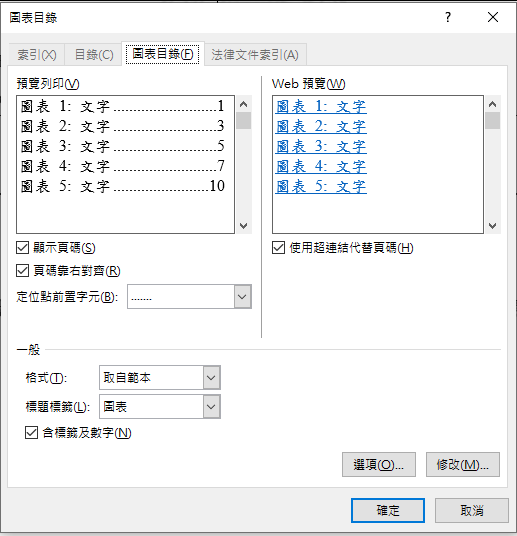
\includegraphics[width=.8\textwidth]{figure3.png}
\caption*{Figure1.3\ 插入圖表目錄}
\addcontentsline{lof}{figure}{Figure1.3\ 插入圖表目錄}
\end{figure}
\clearpage

\section*{第二章\ 新增頁碼與編輯不同類別頁碼}
\addcontentsline{toc}{section}{第二章\ 新增頁碼與編輯不同類別頁碼}

\subsection*{2.1\ 分隔不同頁面以使用不同種類頁碼}
\addcontentsline{toc}{subsection}{2.1\ 分隔不同頁面以使用不同種類頁碼}

\subsubsection*{2.1.1\ 分隔頁面}
\addcontentsline{toc}{subsection}{2.1.1\ 分隔頁面}
為了新增不同種類的頁碼，我們需要先分隔頁面，首先先點擊摘要頁的標題開頭，然後點擊「版面配置」中的「分隔符號」，選擇「下一頁」，如此一來封面和摘要頁的頁碼格式就可以分開來了，同樣的事情在內文的第一頁也須做一次，才能在摘要和圖表目錄間的頁面使用羅馬數字格式的頁碼。
 
\subsubsection*{2.1.2\ 新增頁碼}
\addcontentsline{toc}{subsection}{2.1.2\ 新增頁碼}
接著就是新增頁碼，點選「插入」-「頁碼」，選擇頁碼格式，依據所在頁面選擇符合格式的頁碼種類後，點選「頁面底端」的「純數字2」，就可以新增適合的頁碼到頁面底部。
\clearpage
\input{appendix.tex}

\section*{參考資料}
\addcontentsline{toc}{section}{參考資料}
\subsection*{中原大學官網}
\href{https://www.cycu.edu.tw/}{點擊此處跳轉}\\
\subsection*{中原大學張靜愚紀念圖書館}
\href{https://www.lib.cycu.edu.tw/cycu/Index.action?lang=zh_TW}{點擊此處跳轉}\\
\subsection*{中原大學碩博士論文系統}
\href{https://cloud.ncl.edu.tw/cycu/}{點擊此處跳轉}\\
\subsection*{論文範本電子檔下載(中文範本)}
\href{https://www.lib.cycu.edu.tw/cycu/Fpage.action?muid=436&fid=406&lang=zh_TW&changeLang=true}{點擊此處跳轉}\\
\subsection*{論文範本電子檔下載(英文範本)}
\href{https://www.lib.cycu.edu.tw/cycu/Fpage.action?muid=440&fid=410&lang=en_US&changeLang=true}{Click\ to\ jump}\\
\clearpage

\end{CJK*}
\end{document}
